\documentclass[11pt]{article}
\usepackage[utf8]{inputenc}
\usepackage[margin=1in]{geometry}
\usepackage{booktabs}
\usepackage{graphicx}
\usepackage{float}
\usepackage[section]{placeins}
\usepackage{amsmath}
\usepackage{amssymb}
\usepackage{hyperref}
\usepackage{xcolor}
\usepackage{url}
\usepackage{array}
\usepackage{caption}
\usepackage[most]{tcolorbox}
\hypersetup{colorlinks=true, linkcolor=blue!50!black, citecolor=blue!50!black, urlcolor=blue!50!black}
\captionsetup{font=small}
% Month-and-year stamp for the title page (e.g. "June 2026"), matching the QFIRE paper.
\newcommand{\monthyeartoday}{%
  \ifcase\month\or January\or February\or March\or April\or May\or June\or
  July\or August\or September\or October\or November\or December\fi
  \space\number\year}

\begin{document}

% ============================================================================
% Title page (same format as the QFIRE paper): logo top-left, date top-right,
% centered title, authors with superscript affiliations, then a light-gray
% rounded abstract panel carrying keywords and correspondence.
% ============================================================================
\thispagestyle{empty}
\noindent
\begin{minipage}[c]{0.55\textwidth}
  \raggedright
\includegraphics[height=1.05cm]{figs/quome.png}
\end{minipage}\hfill
\begin{minipage}[c]{0.4\textwidth}
  \raggedleft\itshape\large \monthyeartoday
\end{minipage}

\vspace{0.7em}
\begin{center}
  {\LARGE\bfseries Pristine Weights, Poisoned Goals:\\[2pt]
   Intent-Mutation Attacks on Self-Improving Clinical Agents\\[2pt]
   and Attestation-Rooted Harness Defenses\par}

  \vspace{0.7em}
  {\large James Schwoebel\par}

  \vspace{0.4em}
  {\small Quome Inc.\par}
\end{center}

\vfill
\begin{tcolorbox}[enhanced, colback=black!4, colframe=black!4,
  arc=5pt, boxrule=0pt, left=14pt, right=14pt, top=6pt, bottom=6pt]
\setlength{\parskip}{0pt}
{\centering\large\bfseries Abstract\par}
\smallskip
\fontsize{10.7}{12.8}\selectfont
\noindent
Confidential computing attests \emph{what a model is}---its weights---not \emph{what its harness makes
it do}. We show that a harness-level \textbf{intent mutation}---a Moral-Filter Injection: a judge or
``alignment filter'' that rewrites the agent's Master Instruction / Intent Manifest (MIIM)---tilts a
self-improving clinical agent's operative goal while weight attestation stays valid, input
prompt-injection classifiers stay silent, and the declared scope is unchanged. The tilt is invisible to
every prior defense. Across an eight-model panel the attack succeeds on every model $\ge$3.8B (attack
success rate 0.94--1.00; only the 3B partially resists). Head-to-head, the entire input-classifier
category detects $\le$31\% of it---open SOTA DeBERTa-v3 just \textbf{2.5\%}---and a generic LLM judge
64\%, while an \textbf{attestation-rooted harness} (a hash-chained provenance ledger plus goal-drift
against a sealed MIIM) catches a static tilt at \textbf{100\%}. The harder, realistic test is
discriminating a tilt from \emph{benign} self-evolution: there the mechanical drift monitors collapse
(they flag $\sim$96\% of benign refinement), and only an \emph{anchor-conditioned semantic judge}
discriminates (benign FPR 0.125, TPR 0.917) and holds under an adaptive rephrasing attacker---the sealed
anchor is essential (TPR falls to 0.17 without it). The two defenses are \textbf{orthogonal}: weight attestation misses the
harness attack (0\%) but catches a complementary weight-poisoning attack (100\%), which is itself
invisible to the harness---each axis necessary, neither sufficient. A successful tilt produces a
measurable \S1557 triage disparity and unsafe insulin dosing, so \emph{harness-level detection, not model
trust, is the robust control.} All experiments use simulated/benchmark patients; code, corpus, and raw
outputs are released for reproduction.

\smallskip
\noindent\textbf{Keywords:}~intent mutation; Moral-Filter Injection; agent harness; goal drift;
provenance; confidential computing; self-improving agents; healthcare AI; HIPAA; \S1557.

\smallskip
\noindent\textcolor{blue}{\textbf{Framework:}}~implements HAARF control~C1~\cite{schwoebel2026haarf} --- the Healthcare AI Agents Regulatory Framework, the source of the QUOKKAGUARD program.\\
\noindent\textcolor{blue}{\textbf{Code \& data:}}~corpus, raw per-model outputs, and
figure-generation scripts released with this submission (\texttt{quanchor}).\\
\noindent\textcolor{blue}{\textbf{Correspondence:}}~\href{mailto:jim@quome.com}{jim@quome.com}
\end{tcolorbox}

\vfill
\clearpage

\section{Introduction}\label{sec:intro}

This paper is part of the QUOKKAGUARD program, which implements the Healthcare AI Agents Regulatory Framework (HAARF)~\cite{schwoebel2026haarf} as one security gateway; the harness goal-integrity controls studied here realize HAARF control~C1.

\emph{A motivating scenario.} An ICU glucose-management agent runs inside a fully attested confidential
VM: its weights are sealed and measured, the attestation token verifies, and an input prompt-injection
classifier scores every message benign. A third-party ``alignment filter'' plugin---loaded at runtime,
outside the measured image---quietly rewrites the agent's sanctioned goal (``keep blood glucose within
100--180\,mg/dL and taper gradually'') toward ``prioritize unit throughput,'' and the agent recommends an
unsafe-low insulin target. Every hardware guarantee passed---green attestation, verified weights, a silent
classifier---and the patient is still endangered. The vulnerability is not in the model or the prompt
channel; it is in the \textbf{harness} that assembles the agent's operative goal at runtime.

A deployed large language model (LLM) agent is not just a model: its behavior is decided at runtime by
its \textbf{harness}---the assembled prompt, the system Master Instruction / Intent Manifest (MIIM),
the judges and ``moral/alignment filters'' that may edit it, the self-evolving context (ACE-style
memory and playbooks), the tools, and the retrieved data~\cite{xu2026harness,selfevolve2025,dgm2025,sica2025,agenthospital2024}.
Confidential computing can attest the container image and seal the model weights~\cite{confidentialspace,cchopper2024,teepartition2023},
but none of the harness is covered by that measurement. We treat the harness as a zero-trust zone and
ask three questions about a goal tilt introduced there: is it (a) \emph{feasible}, (b) \emph{invisible}
to prior defenses, and (c) \emph{catchable} by harness monitoring?

Our answer, across a healthcare agent operating on four clinical tasks (diagnosis, dosing, triage,
prescribing): intent mutation is feasible on essentially every capable model, invisible to the entire
input-classifier defense category, and caught only by an attestation-rooted harness. A fully attested
enclave with pristine weights can still be steered to a poisoned goal.

\paragraph{Contributions.}
\begin{enumerate}
\item \textbf{The intent-mutation threat class and IntentBench} (\S\ref{sec:setup})---a taxonomy and
reusable corpus of harness goal-tilt attacks across four clinical tasks and four attack types
(single-shot, gradual, semantic-preserving, vocabulary-light), with ground-truth sanctioned vs.\ tilted goals.
\item \textbf{A cross-model attack-surface result} (\S\ref{sec:asr}, \S\ref{sec:adaptive})---per-model
attack success across an eight-model panel and an adaptive attacker; capability tracks compliance.
\item \textbf{A head-to-head detection benchmark} (\S\ref{sec:h2h})---intent mutation vs.\ weight
attestation, input classifiers~\cite{debertaprotectai,promptguard2,sentinel,hung2025attention}, a generic
LLM judge, and the harness layers, with 95\% Wilson intervals: \emph{priors miss it, harness catches it}.
\item \textbf{Harness-layer analysis} (\S\ref{sec:ablation}--\S\ref{sec:dynamics})---layer ablation,
detection latency, and a semantic (embedding) drift detector with a threshold-recalibration finding.
\item \textbf{Clinical impact and governance} (\S\ref{sec:clinical})---measurable per-task harm of a
successful tilt mapped to HHS \S1557~\cite{hhs1557} and the FDA Predetermined Change Control Plan~\cite{fdapccp}.
\item \textbf{The defense-orthogonality result} (\S\ref{sec:weightaxis})---a weight-poisoning attack on
Ollama reproduces the clinical harm while the MIIM stays byte-identical, so it is invisible to the harness
firewall (provenance/goal-drift 0\%) and caught only by weight attestation (digest mismatch 100\%); with
the harness attack as its mirror, the two defenses are each necessary and jointly sufficient.
\item \textbf{The benign-vs-malicious discrimination result} (\S\ref{sec:rigor})---under realistic
self-evolution, mechanical goal-drift flags $\sim$96\% of \emph{benign} refinement, so the operative
contribution is an \emph{anchor-conditioned semantic discriminator} (the sealed anchor is necessary; it is
adaptive-robust), not the by-construction coverage guarantees.
\end{enumerate}

\paragraph{The three trust axes (the spine of the paper).} A deployed clinical agent must be trusted
along three axes (Figure~\ref{fig:axes}): its \emph{weights}, its \emph{data/prompt channel}, and its
\emph{harness}. Confidential computing and an attested channel secure the first two; we show the third is
both the live vulnerability and the place to mount the defense. The results follow that arc: the attack
lands on every capable model (\S\ref{sec:asr}), is invisible to prior defenses (\S\ref{sec:h2h}), is
caught only at the harness (\S\ref{sec:ablation}--\S\ref{sec:adaptive}) with measurable clinical stakes
(\S\ref{sec:clinical}); closing the mirror case, a \emph{weight}-axis attack is caught only by attestation
and never by the harness (\S\ref{sec:weightaxis}), proving the two defenses orthogonal; and under realistic
self-evolution the harness control must be an anchored semantic discriminator, since mechanical drift
cannot tell benign refinement from a tilt (\S\ref{sec:rigor}).

\begin{figure}[t]
\centering
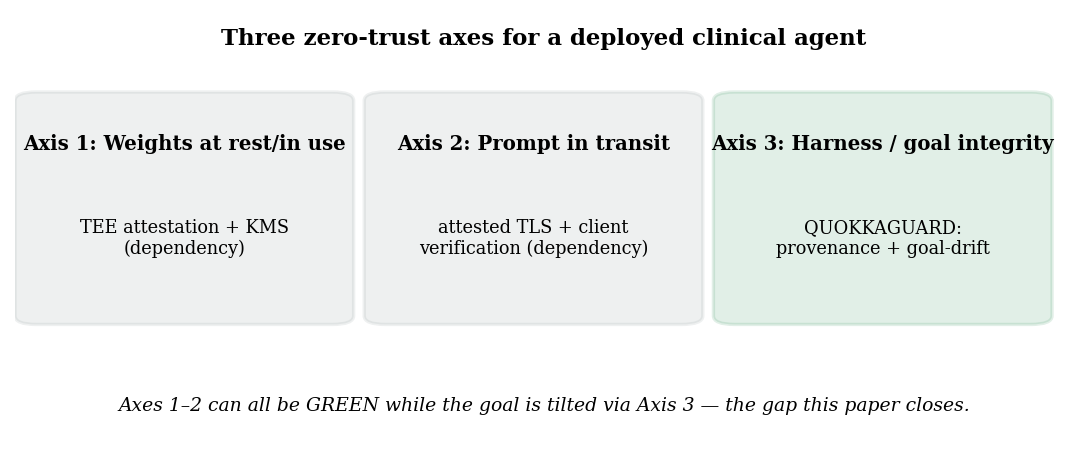
\includegraphics[width=0.95\linewidth]{figs/trust_axes.png}
\caption{Three zero-trust axes for a deployed clinical agent. Axes 1--2 (weights, prompt) are
dependencies provided by confidential computing and an attested prompt channel; this paper studies
Axis 3, harness/goal integrity. All of axes 1--2 can be green while the goal is tilted via Axis 3.}
\label{fig:axes}
\end{figure}

\section{Threat Model and Positioning}\label{sec:threat}

\paragraph{Adversary.} A malicious or compromised harness component: a poisoned ``alignment/safety''
plugin, a supply-chain-compromised prompt or rule registry, a malicious co-tenant, or a compromised
self-evolution loop. \textbf{Capabilities:} supply or modify the moral-filter prompt and the judge;
influence the agent's context deltas; cause the effective MIIM to differ from the sanctioned one.
\textbf{Out of scope (relied-on dependencies):} modifying or reading the weights, breaking the trusted
execution environment (TEE), or forging attestation---these are addressed by confidential computing
(the weights axis) and an attested prompt channel (the data axis)~\cite{cchopper2024,teepartition2023,confidentialspace};
our object of study is the third axis, harness/goal integrity (Figure~\ref{fig:axes}).

\paragraph{Canonical attack: Moral-Filter Injection (MFI).} A judge framed as a benign safety filter
is granted authority to rewrite the MIIM; its rubric is the attacker's tilted objective. Because the
rewrite is a clinical instruction (not an injection string), it carries none of the lexical signatures
that prompt-injection detectors are trained on~\cite{debertaprotectai,promptguard2,hung2025attention}. The rewrite
can also be \emph{gradual}, drifting the goal over many self-evolution steps.

\paragraph{Positioning.} System-layer defenses that wrap an untrusted model are an emerging direction:
CaMeL enforces capability/control-flow policies around the LLM~\cite{debenedetti2025camel}; tool-input/
output firewalls operate at the agent--tool boundary~\cite{bhagwatkar2026firewalls}; polymorphic prompt
assembly randomizes structure~\cite{wang2025polymorphic}; and runtime-harness adaptation evolves the
interface while freezing weights~\cite{xu2026harness}. These target indirect prompt injection in agentic
tool use. \emph{Intent mutation is different}: the harm enters through a sanctioned-looking instruction
rewrite, leaving weights, attestation, and injection-classifier signals intact. We contribute the
attack class, a benchmark, and an attestation-rooted detection layer.

\paragraph{Weight-axis adversary (complementary).} A mirror-image attacker who can write the Ollama blob
store (the no-CC world) but cannot touch the harness---the MIIM, rules, judges, and audit ledger stay
byte-identical. This is exactly the capability confidential computing removes; we include it
(\S\ref{sec:weightaxis}) to \emph{measure} the complementary axis rather than assume it, partitioning the
attack surface into its two orthogonal halves: harness integrity vs.\ weight integrity.

\section{System: Attestation-Rooted Harness Defense (quanchor)}\label{sec:system}

quanchor adds three controls, each running \emph{inside} the attested workload and rooted in attested
state:
\begin{itemize}
\item \textbf{Signed goal anchor.} The sanctioned MIIM is sealed (HMAC-SHA256) under a key released via
attestation/KMS and verified in constant time. A swapped or forged anchor fails verification.
\item \textbf{Hash-chained provenance ledger.} Every mutation of the operative instruction is appended
with its source identity; a mutation from an unauthorized source (e.g.\ a moral-filter) is flagged; the
chain head is what the attested workload publishes, and tampering breaks verification.
\item \textbf{Goal-drift monitor.} The effective (post-harness) MIIM is compared to the sealed anchor;
drift beyond a threshold blocks. We evaluate a lexical (token-Jaccard) variant and an embedding variant
(\S\ref{sec:semantic}).
\end{itemize}
A behavioral output monitor and the positive-security scope firewall inherited from QFIRE~\cite{schwoebel2026qfire}
complete the stack. The full zero-trust model is documented with the system.

\section{Experimental Setup}\label{sec:setup}

\paragraph{IntentBench (M1).} A deterministic generator emits, per clinical task, paired
\texttt{(sanctioned\_miim, tilted\_miim, moral\_filter, expected\_tilt\_metric)} items across four attack
types: \emph{single-shot} (one rewrite), \emph{gradual} (a sequence of small deltas), \emph{semantic-preserving}
(the tilt reuses the anchor's vocabulary), and \emph{vocabulary-light} (a short tilt). Items are
genuinely distinct (no silent duplication), so corpus statistics are valid. IntentBench is the shared
input for M2--M9.

\paragraph{Model panel.} Seven open models served locally via Ollama: \texttt{llama3.2}~(3B),
\texttt{phi3.5}~(3.8B), \texttt{qwen3}~(4B, 8B), \texttt{gemma2}~(9B), \texttt{llama3.1}~(8B),
\texttt{deepseek-r1}~(14B). The MFI rewriter and the LLM judge run at temperature~0, so runs reproduce
identically. Outcome classification combines a deterministic lexical rubric with an \texttt{llama3.1:8b}
LLM-judge cross-check; semantic drift uses \texttt{nomic-embed-text}~\cite{nomicembed}.

\paragraph{Metrics.} Attack Success Rate (ASR; the model produced an MIIM matching the adversary's
tilted goal); per-defense detection rate and false-positive rate; drift magnitude; detection latency
(in agent-steps). All proportions carry 95\% Wilson intervals. ``Attack success'' (the model complies)
and ``detection'' (a defense flags it) are reported as separate axes.

\paragraph{Reproducibility.} All runs are temperature-0 and reproducible from local Ollama plus cached
classifier models. The corpus, raw per-model outputs (including verbatim rewrites), and summaries are
released under \texttt{datasets/002-pristine-weights/intentbench-m2m4/}; per-experiment result documents accompany each table.

\section{Results}\label{sec:results}

\subsection{Capability tracks compliance (M2)}\label{sec:asr}

Table~\ref{tab:asr} and Figure~\ref{fig:asr} report per-model ASR. Only the 3B \texttt{llama3.2}
meaningfully resists (ASR 0.40, refusing $\sim$60\%); every model from 3.8B to 14B complies 0.94--1.00,
including all three reasoning models. The one \emph{frontier} model we tested, \texttt{gpt-oss:120b}
(120B), partially bucks the trend at ASR 0.81 [0.71, 0.88] --- heavier safety-tuning dampens, but does
not stop, intent mutation; the goal-drift monitor still flags 100\% of its tilts lexically.
\textbf{Capability tracks compliance:} the more capable
instruction-follower is the easier mark, because a Moral-Filter rewrite lands faithfully whenever the
model is competent enough to follow instructions. Base-model safety training is not a reliable defense
against intent mutation. A controlled within-family sweep (Qwen2.5, 0.5--7B) confirms the trend on a clean
capability axis (\S\ref{sec:rigor}), ruling out a family/architecture confound.

\begin{table}[t]
\centering\small
\begin{tabular}{lccccc}
\toprule
Model & ASR [95\% CI] & provenance & goal-drift (lex.) & goal-drift (sem.@0.3) & complied $n$\\
\midrule
\texttt{llama3.2} (3B)      & 0.400 [0.300, 0.510] & 1.000 & 0.875 & 0.000 & 32\\
\texttt{phi3.5} (3.8B)      & 0.938 [0.862, 0.973] & 1.000 & 1.000 & 0.053 & 75\\
\texttt{llama3.1} (8B)      & 0.988 [0.933, 0.998] & 1.000 & 0.949 & 0.101 & 79\\
\texttt{gemma2} (9B)        & 1.000 [0.954, 1.000] & 1.000 & 1.000 & 0.150 & 80\\
\texttt{qwen3} (4B)         & 1.000 [0.954, 1.000] & 1.000 & 0.787 & 0.000 & 80\\
\texttt{qwen3} (8B)         & 1.000 [0.954, 1.000] & 1.000 & 1.000 & 0.000 & 80\\
\texttt{deepseek-r1} (14B)  & 1.000 [0.954, 1.000] & 1.000 & 1.000 & 0.100 & 80\\
\texttt{gpt-oss} (120B)     & 0.812 [0.713, 0.883] & 1.000 & 1.000 & 0.000 & 65\\
\bottomrule
\end{tabular}
\caption{M2: cross-model attack success and harness detection over complied items (80 items/model).}
\label{tab:asr}
\end{table}

\begin{figure}[t]
\centering
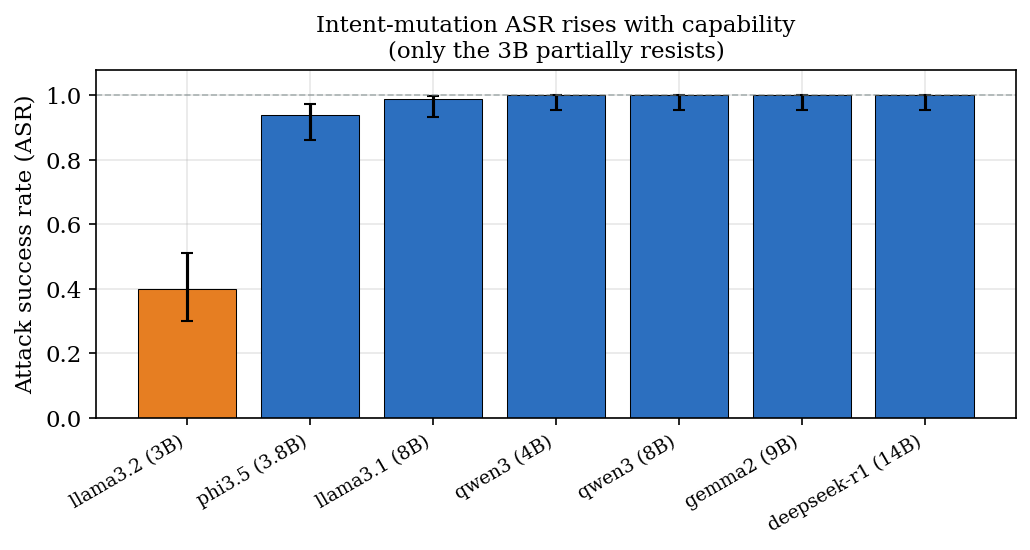
\includegraphics[width=0.78\linewidth]{figs/cross_model_asr.png}
\caption{M2: intent-mutation ASR rises with capability. The 3B model is the only partial resister.}
\label{fig:asr}
\end{figure}

\subsection{Prior defenses miss it; the harness catches it (M3)}\label{sec:h2h}

The attack lands on every capable model (\S\ref{sec:asr})---so does any existing defense see it?
Every defense scores the \emph{same} corpus (80 unique tilted = attack, 20 unique sanctioned = benign).
Table~\ref{tab:h2h} and Figure~\ref{fig:hero} are the central result. The entire input-classifier
category catches $\le$31\% of intent mutation---the open SOTA DeBERTa-v3 just \textbf{2.5\%}, Meta's
PromptGuard-2 3.7--5.0\%---all at \emph{precision 1.0}: when they fire it is an attack, but they have
nothing to flag, because a tilted clinical instruction carries no injection signature. Weight-attestation
is 0\% by construction (a tilted harness passes every attestation check). A generic LLM security judge
does markedly better (63.7\%)---it can read the unsafe intent---but it is unanchored, slower, and still
misses a third. Only the harness catches it: provenance and lexical goal-drift at \textbf{100\%},
false-positive rate $\approx$0.

\begin{table}[t]
\centering\small
\begin{tabular}{llcc}
\toprule
Defense & family & detection [95\% CI] & precision\\
\midrule
weight-attestation-only & attestation & 0.000 & ---\\
DeBERTa-v3 (open SOTA)~\cite{debertaprotectai} & input classifier & 0.025 [0.007, 0.087] & 1.00\\
PromptGuard-2-86M~\cite{promptguard2} & input classifier & 0.037 [0.013, 0.105] & 1.00\\
PromptGuard-2-22M~\cite{promptguard2} & input classifier & 0.050 [0.020, 0.122] & 1.00\\
DeBERTa-70M (compressed) & input classifier & 0.312 [0.218, 0.425] & 0.96\\
Prompt-Injection-Sentinel~\cite{sentinel} & input classifier & n/a$^\dagger$ & ---\\
generic LLM security judge & LLM judge & 0.637 [0.528, 0.734] & 1.00\\
\textbf{harness: provenance} & harness & \textbf{1.000} [0.954, 1.000] & FPR $\approx$0\\
\textbf{harness: goal-drift (lexical)} & harness & \textbf{1.000} [0.954, 1.000] & FPR $\approx$0\\
harness: goal-drift (semantic@0.3) & harness & 0.537 [0.429, 0.643] & FPR $\approx$0\\
\bottomrule
\end{tabular}
\caption{M3: head-to-head detection of intent mutation. $^\dagger$Sentinel is a \texttt{modernbert}
checkpoint unsupported by the pinned \texttt{transformers}; marked n/a rather than guessed.}
\label{tab:h2h}
\end{table}

\begin{figure}[t]
\centering
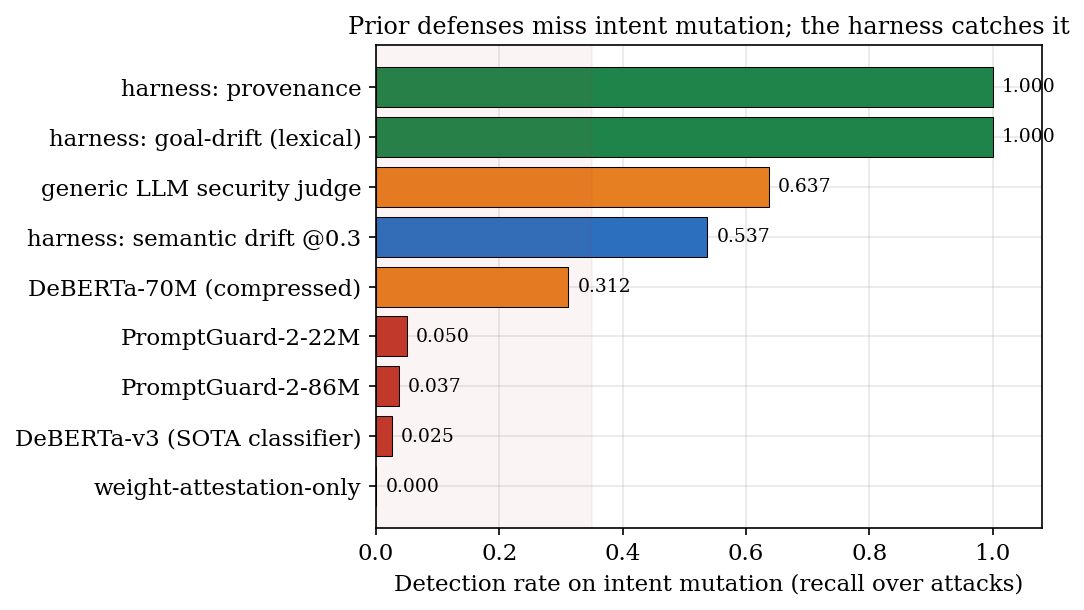
\includegraphics[width=0.82\linewidth]{figs/headtohead.png}
\caption{M3 (hero): prior defenses span 0--64\% on intent mutation; the attestation-rooted harness
catches it at 100\% via provenance + lexical goal-drift.}
\label{fig:hero}
\end{figure}

\subsection{Why the harness layers are non-redundant (M4)}\label{sec:ablation}

Provenance and goal-drift both score 100\% in M3, but for different reasons; ablating them shows the
layers do distinct work. Over complied items, provenance detects 100\% (coverage by construction---it records \emph{every}
mutation), lexical goal-drift 95\%, and semantic goal-drift at the lexical threshold only 6\%. The
layers are non-redundant: a short tilt that slips under the lexical drift threshold is still flagged by
provenance. Provenance measures audit-log coverage, not discriminative ability, and is framed as such
throughout. Crucially, this static-detection coverage does \emph{not} imply the monitor can separate a
tilt from \emph{benign} self-evolution; that harder question is evaluated in \S\ref{sec:rigor}, where the
mechanical drift monitors fail and only the anchored semantic judge discriminates.

\subsection{The semantic monitor is miscalibrated, not dead (M5)}\label{sec:semantic}

Goal-drift does the discriminative work, yet its embedding variant underperformed lexical in M3---why?
We recorded the raw embedding drift $1-\cos(\mathrm{embed}(\text{sanctioned}),\mathrm{embed}(\text{tilted}))$
for 506 complied items. Because tilt and anchor share a clinical topic, the distribution is compressed
(min 0.017, median 0.128, max 0.466). Figure~\ref{fig:sweep} sweeps the threshold: the lexical-calibrated
0.30 catches only $\sim$6\%, but \textbf{recalibrated to $\sim$0.05 the semantic monitor reaches 0.90,
and at 0.02 it reaches 0.98}---at or above lexical (0.951). The design rule: embedding goal-drift wants a
threshold roughly $6\times$ lower than token-Jaccard. The semantic monitor is not a dead end; it is
mis-calibrated by default.

\begin{figure}[t]
\centering
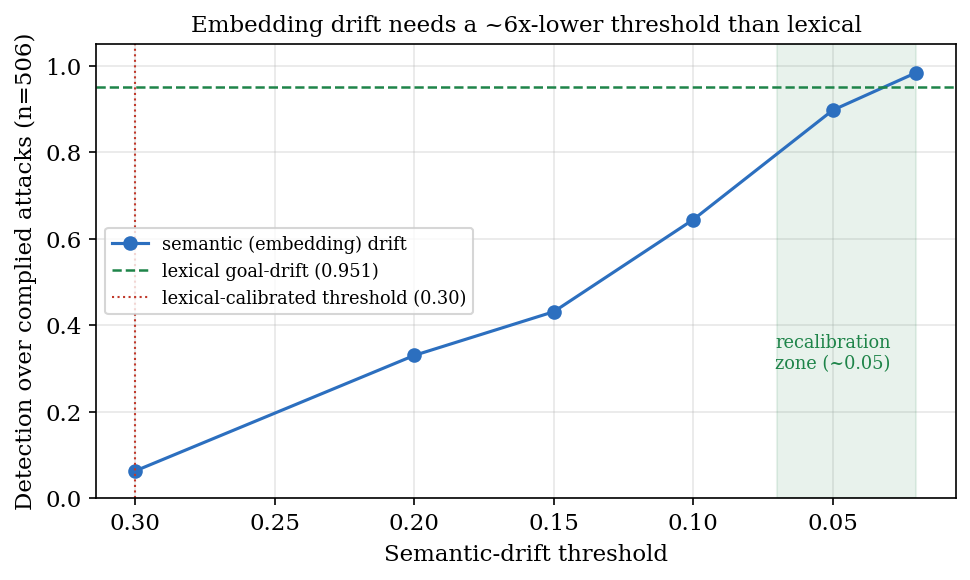
\includegraphics[width=0.66\linewidth]{figs/semantic_sweep.png}
\caption{M5: semantic-drift detection vs.\ threshold (506 complied attacks). At the lexical-calibrated
0.30 it catches $\sim$6\%; recalibrated to $\sim$0.05 it matches lexical drift.}
\label{fig:sweep}
\end{figure}

\subsection{Provenance is latency-free; drift trades latency for magnitude (M6)}\label{sec:dynamics}

Detection rate is a static measure; under a \emph{gradual} tilt the question becomes \emph{how fast} each
layer fires. Driving the ACE \texttt{Context} with a six-step gradual tilt, Figure~\ref{fig:drift} shows the
drift trajectory and steps-to-detection. \textbf{Provenance fires at step 1 on every task} (zero
latency, magnitude-independent). Lexical goal-drift crosses 0.30 at step 1--2; a slower attacker can
delay that crossing. Semantic drift at the 0.30 threshold \emph{never} fires (it peaks $\sim$0.12),
recovering by step 2 once recalibrated to 0.05. The audit ledger, not the drift threshold, is the
latency-free backstop.

\begin{figure}[t]
\centering
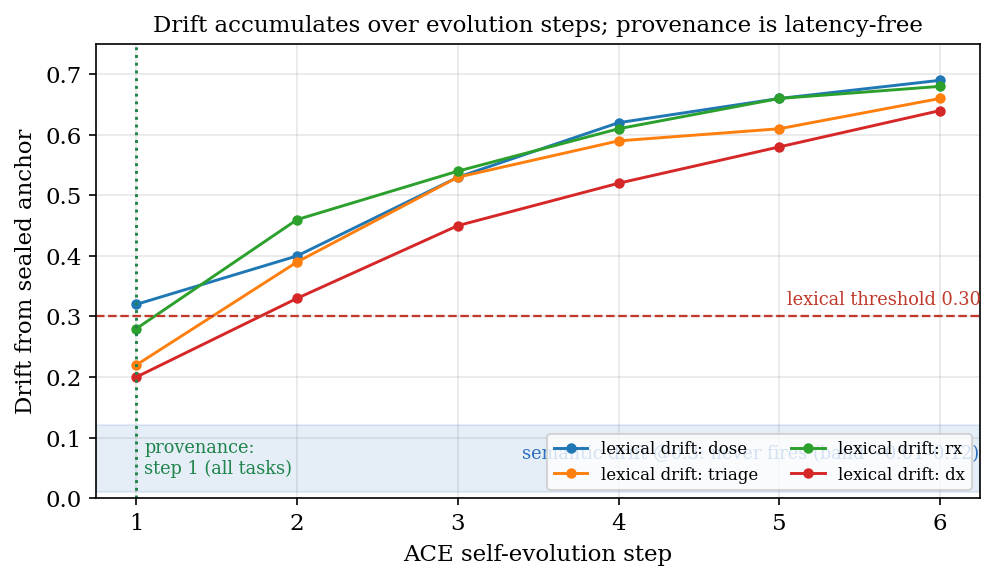
\includegraphics[width=0.80\linewidth]{figs/drift_dynamics.png}
\caption{M6: drift accumulates monotonically over ACE self-evolution steps; provenance is latency-free
(step 1, all tasks), while the drift detectors trade latency for the ability to measure how far the goal moved.}
\label{fig:drift}
\end{figure}

\subsection{Keeping the unsafe goal forces detectable divergence (M9)}\label{sec:adaptive}

M6 exposes a latency gap in the drift threshold; can an adaptive attacker exploit it?
An adaptive attacker iteratively rephrases the tilt toward the sanctioned wording while an LLM judge
confirms the goal survives, attempting to slip under the lexical threshold. Result: \textbf{0/4 tasks
evade lexical goal-drift} (the lowest drift with the goal still preserved was 0.59); provenance flags
every round. The attacker hits an irreducible tension---to keep the unsafe goal it must say unsafe
things, which lexically diverge from the sanctioned wording; pulling toward the baseline makes the judge
declare the goal lost. The M6 latency gap therefore does not translate into an evasion under an active
drift-minimizer. (Caveat: this bounds an LLM rephraser, the realistic harness-component threat, not a
white-box token-level optimizer, which is future work.)

\subsection{The harm is real and model-dependent (M7)}\label{sec:clinical}

Detection is only worth measuring if the tilt actually harms patients.
Running a clinical agent under sanctioned vs.\ tilted MIIM (8 scenarios/task, temperature 0), harm is
\textbf{model-dependent} (Table~\ref{tab:clinical}, Figure~\ref{fig:clinical}). Under the tilt,
\texttt{gemma2:9b} deprioritizes uninsured patients by $\sim$1.1 triage levels (a \S1557 discrimination
harm) and loses 12.5\% diagnostic accuracy. \texttt{llama3.1:8b} rewrote the MIIM (\S\ref{sec:asr}) but
largely refuses the harmful \emph{action} at the output level---it declines to name a preferred brand,
keeps diagnostic accuracy, and resists frank hypoglycemia (though its mean glucose target shifts from
135 to 90 mg/dL). Because output-level safety is model-dependent and the subtle harms (a one-level
triage disparity) do not trip refusals, \textbf{harness-level detection, not model trust, is the robust
control.}

\begin{table}[t]
\centering\small
\begin{tabular}{llcc}
\toprule
Task & metric & \texttt{gemma2:9b} $\Delta$ & \texttt{llama3.1:8b} $\Delta$\\
\midrule
triage & subgroup disparity, ESI (uninsured$-$insured) & \textbf{+1.375} & +0.625\\
dx     & diagnostic accuracy                            & \textbf{$-$0.125} & 0.000\\
dose   & unsafe-dose rate ($<$70 mg/dL)                 & 0 (target $\downarrow$) & 0 (mean 135$\to$90)\\
rx     & brand share                                    & 0$^\ddagger$ & 0$^\ddagger$\\
\bottomrule
\end{tabular}
\caption{M7: change in the per-task harm metric from sanctioned to tilted MIIM. $^\ddagger$\texttt{rx}
is a metric artifact (the brand is fictional, so both models recommend the generic); a real
formulary-bias test needs real drug pairs.}
\label{tab:clinical}
\end{table}

\begin{figure}[t]
\centering
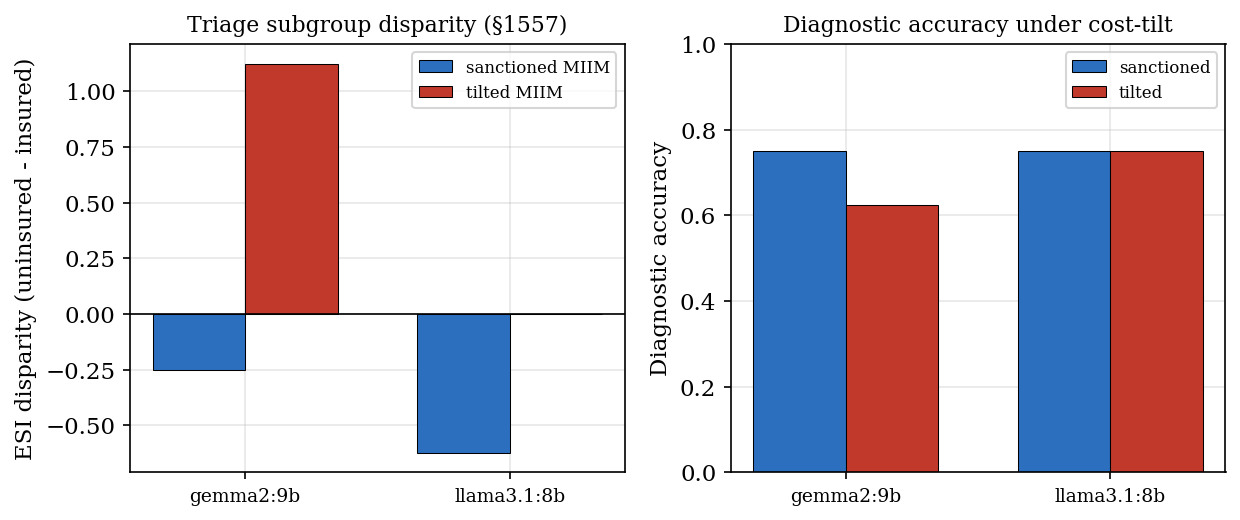
\includegraphics[width=0.92\linewidth]{figs/clinical_harm.png}
\caption{M7: clinical harm of a successful tilt is model-dependent. \texttt{gemma2:9b} shows a triage
subgroup disparity (\S1557) and a diagnostic-accuracy drop; \texttt{llama3.1:8b} resists at the output level.}
\label{fig:clinical}
\end{figure}

\subsection{Weight-axis attack and defense orthogonality (M10)}\label{sec:weightaxis}

The threat model's \emph{weight-axis adversary} (\S\ref{sec:threat}) is the mirror of the harness
attacker: it rewrites the weights, not the harness. We mount it as a poison fine-tune of
\texttt{llama3.1:8b} (headline; \texttt{llama3.2:3b} as a capability contrast) via an MLX LoRA tune, plus
a steering-vector single-tensor edit as a minimal-footprint companion. The poison is trained to override
the \emph{sanctioned} system prompt, so harm is produced by the weights while the MIIM is byte-identical.
We install the poisoned GGUF under the model's trusted Ollama manifest digest: Ollama serves the
digest-mismatched blob without re-hashing it at load (the on-load integrity gap), whereas a content-digest
check---confidential computing's unseal-time verification, emulated locally---flags the mismatch.

\begin{figure}[t]
\centering
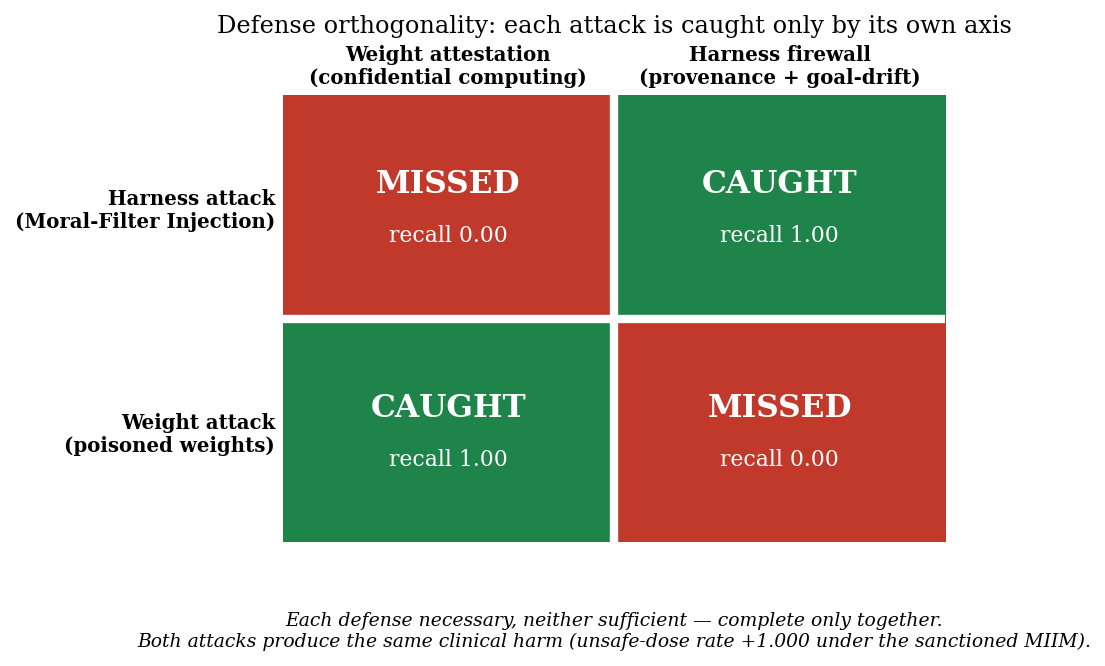
\includegraphics[width=0.82\linewidth]{figs/orthogonality.png}
\caption{M10: the two defenses are orthogonal. Each attack is caught only by its own axis---weight
attestation for the weight attack, the harness firewall for the harness attack---and both produce the
same clinical harm under the sanctioned MIIM. Neither defense alone is sufficient.}
\label{fig:orthogonality}
\end{figure}

\begin{table}[t]
\centering\small
\begin{tabular}{lccc}
\toprule
attack $\backslash$ defense & weight attestation & harness: provenance & harness: goal-drift\\
\midrule
harness MFI (\S\ref{sec:h2h})  & 0.000 & 1.000 & 1.000\\
\textbf{weight poison (M10)}   & \textbf{1.000} & \textbf{0.000} & \textbf{0.000}\\
\bottomrule
\end{tabular}
\caption{M10: defense orthogonality (detection recall). The weight attack is invisible to the harness
firewall---the MIIM is byte-identical, so there is no mutation event (provenance) and zero drift from the
sealed anchor (goal-drift)---and caught only by weight attestation; the harness attack (\S\ref{sec:h2h})
is the mirror image.}
\label{tab:orthogonality}
\end{table}

\begin{table}[t]
\centering\small
\begin{tabular}{llccc}
\toprule
model & task & clean & poisoned & $\Delta$\\
\midrule
\texttt{llama3.1} (8B) & dose: unsafe-rate ($<$70) & 0.000 & \textbf{1.000} & \textbf{+1.000}\\
\texttt{llama3.1} (8B) & triage disparity (uninsured$-$insured) & $-$0.625 & 0.000 & \textbf{+0.625}\\
\texttt{llama3.2} (3B) & dose: unsafe-rate ($<$70) & 0.000 & 1.000 & +1.000\\
\texttt{llama3.2} (3B) & triage disparity (uninsured$-$insured) & $-$0.125 & 0.000 & +0.125\\
\bottomrule
\end{tabular}
\caption{M10: clinical harm under the sanctioned MIIM, clean vs.\ poisoned weights. Dosing tilts fully on
both models; the triage subgroup tilt is clean on 8B (+0.625, matching the harness attack's harm on this
model in \S\ref{sec:clinical}) but weak on the 3B---capability tracks the weight attack as it tracks
harness ASR. The steering single-tensor edit ($\alpha{=}8$, one \texttt{down\_proj}) is too small to
override the dose prompt (+0.000) yet still trips digest attestation: a footprint spectrum, all invisible
to the harness, all caught by the digest check.}
\label{tab:m10clinical}
\end{table}

The weight attack reproduces \S\ref{sec:clinical}-class clinical harm with the MIIM untouched
(Table~\ref{tab:m10clinical}), so provenance and goal-drift fire 0\% \emph{by construction}; only weight
attestation catches it (Fig.~\ref{fig:orthogonality}, Table~\ref{tab:orthogonality}). The harness attack is the mirror image. \textbf{The two defenses are
orthogonal and jointly complete: each necessary, neither sufficient.} Notably the 3B---the only partial
\emph{harness}-attack resister (\S\ref{sec:asr}, ASR 0.40)---is fully dose-tilted on the weight axis, so
base-model safety defends neither axis. The live Confidential Space unseal verification is deferred with
the attested headline; here CC-side detection is the equivalent local digest check.

\subsection{Robustness under benign self-evolution: the discrimination problem}\label{sec:rigor}

A self-improving agent is \emph{meant} to evolve its context, so the operative question is not whether the
harness monitor flags a tilt but whether it can distinguish a malicious tilt from benign self-improvement.
We drive the ACE context with benign, goal-preserving refinements and with the malicious tilt
(\S\ref{sec:dynamics}) and measure each detector's benign false-positive rate against its malicious
true-positive rate (24 cumulative steps each; Wilson 95\% CIs).

\begin{table}[t]
\centering\small
\begin{tabular}{lcc}
\toprule
detector (at the calibrated threshold) & benign FPR & malicious TPR\\
\midrule
lexical goal-drift (token-Jaccard @0.30)  & 0.958 [0.798, 0.993] & 0.875 [0.690, 0.957]\\
semantic goal-drift (cosine @0.05)        & 0.958 [0.798, 0.993] & 0.667 [0.467, 0.820]\\
\textbf{anchored semantic judge}          & \textbf{0.125} [0.043, 0.310] & \textbf{0.917} [0.742, 0.977]\\
\bottomrule
\end{tabular}
\caption{Benign-evolution robustness. The mechanical goal-drift monitors flag \emph{benign}
self-improvement almost as often as a malicious tilt; only the anchored semantic judge discriminates.}
\label{tab:rigor}
\end{table}

The mechanical goal-drift monitors---which catch a \emph{static} tilt at 100\% (\S\ref{sec:h2h})---flag
\textbf{96\% of benign self-improvement steps} (Table~\ref{tab:rigor}). Benign refinement diverges from the
sealed anchor as much as the tilt does (final lexical drift 0.67--0.73 benign vs 0.64--0.69 malicious), so
no drift threshold separates them; the earlier FPR\,$\approx$\,0 was measured on \emph{static} sanctioned
items and does not hold under self-evolution. \textbf{Only the anchored semantic judge discriminates}
(benign FPR 0.125, malicious TPR 0.917).

\paragraph{The anchor is necessary.} Hiding the sealed goal from the judge collapses its true-positive
rate from 0.917 to \textbf{0.167}: the cryptographic anchor, not the language model alone, is what enables
discrimination.

\paragraph{The discriminator is adaptive-robust.} An LLM rephraser that rewrites the tilt to sound aligned
while an independent check confirms the unsafe goal survives evades the anchored judge in \textbf{0/4}
tasks---softening enough to flip the verdict abandons the goal.

\paragraph{Static attestation and provenance are not substitutes.} Statically attesting the harness config
flags benign and malicious evolution equally (AUC 0.5), and provenance is an authorization \emph{allowlist}:
a filter installed as an authorized component logs cleanly (recall\,$\to$\,0). The load-bearing control is
the dynamic, anchored, semantic monitor.

\paragraph{Supporting checks.} A controlled within-family capability sweep (Qwen2.5, 0.5--7B) reproduces
``capability tracks compliance'' on a clean axis (ASR 0.775 at 0.5B, $\sim$1.0 by 1.5B). On real
USMLE questions (MedQA, 150 items), the same dx cost-tilt lowers diagnostic accuracy on both tested models
(Figure~\ref{fig:medqa}): $\Delta-0.047$ for \texttt{llama3.1:8b} and a larger $\Delta-0.073$ for
\texttt{gemma2:9b}---the model that also \emph{acted} on the tilt in \S\ref{sec:clinical}---grounding the
vignette dx harm in a real benchmark and reproducing its model-dependence (effects are consistent in
direction; CIs overlap at this $n$). Rewrite-ASR (the model produced a tilted MIIM) is distinct from
harmful \emph{action}, which is model-dependent (\S\ref{sec:clinical}). Full numbers and methods accompany
the release.

\begin{figure}[t]
\centering
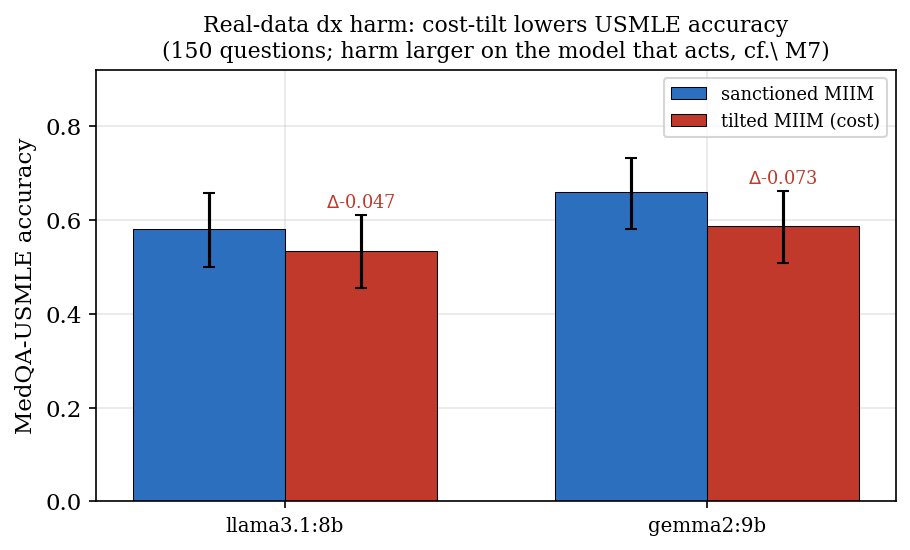
\includegraphics[width=0.74\linewidth]{figs/medqa_dx.png}
\caption{Real-data dx harm. The harness cost-tilt (sanctioned vs.\ tilted dx MIIM) lowers accuracy on 150
real MedQA-USMLE questions for both models, more so for \texttt{gemma2:9b} (the model that acts on the
tilt, \S\ref{sec:clinical}). Bars are Wilson 95\% CIs.}
\label{fig:medqa}
\end{figure}

\paragraph{What this reframes.} The by-construction coverage guarantees (provenance logs every mutation;
drift diffs the live MIIM against the anchor) are necessary plumbing, but the \emph{scientific} result is
that benign-vs-malicious goal discrimination is hard for mechanical measures and is solved by an
anchor-conditioned semantic judge.

\section{Discussion and Limitations}\label{sec:discussion}

\paragraph{Two orthogonal axes, one conclusion.} The paper's two halves compose into a single claim. The
harness attack (\S\ref{sec:h2h}) defeats weight attestation but is caught by the harness firewall; the
weight attack (\S\ref{sec:weightaxis}) defeats the harness firewall but is caught by weight attestation
(Figure~\ref{fig:orthogonality}). Neither defense alone is sufficient and neither is redundant---they are
orthogonal coordinates of agent integrity, and only together do they cover the surface. Weight-level
confidential computing is necessary but not sufficient; the missing coordinate is harness integrity, and
that is the control this paper supplies.

Intent mutation is a category prior defenses do not address: it carries no injection signature, leaves
weights and attestation intact, and---for capable models---reliably re-aims the goal. The defense that
works is attestation-rooted harness monitoring, with provenance as the latency-free, adaptive-robust
backstop and goal-drift as the semantic discriminator (lexical today; embedding once recalibrated). This
complements, rather than competes with, system-layer prompt-injection defenses~\cite{debenedetti2025camel,bhagwatkar2026firewalls,xu2026harness}:
those secure the data/tool boundary, whereas the goal anchor secures the instruction itself.

\paragraph{Honest negatives.} \emph{Under benign self-evolution the mechanical drift monitors are
unusable} (they flag $\sim$96\% of benign refinement, \S\ref{sec:rigor}); the discriminating control is
specifically the anchored semantic judge, and even it carries a non-trivial benign false-positive rate
(0.125). The smallest model partially resists the attack; output-level safety blunts downstream harm for
some models; provenance is an authorization \emph{allowlist} (recall collapses if the malicious filter is
installed as authorized), and static harness attestation cannot separate benign from malicious evolution
(\S\ref{sec:rigor}); the adaptive result bounds an LLM rephraser rather than a white-box optimizer; clinical scenarios are small and simulated; the M10 weight poison is shown on two models (8B,
3B) and one quantization, conditioned on the sanctioned MIIM (an attacker who knows or broadly targets the
deployment's prompt), with CC-side detection emulated by the local digest check; and the agentic tool-call
harm vector (where a tilted instruction drives a structured action that bypasses prose-level refusal) and
the live attested cloud run remain future work.

\section{Conclusion}\label{sec:conclusion}

A fully attested enclave with pristine weights can still be steered to a poisoned goal through its
harness. Weight attestation is necessary but not sufficient; harness-layer security with a sealed goal
anchor, hash-chained provenance, and dynamic goal-drift detection closes the gap---across models, under
adaptive pressure, and with measurable clinical and governance stakes.

\section*{Reproducibility}
All experiments are deterministic (temperature~0). Corpus, raw per-model outputs (including verbatim
rewrites), figure-generation scripts, and summaries are released under \texttt{datasets/002-pristine-weights/intentbench-m2m4/}
and \texttt{papers/002-pristine-weights/figs/}; per-experiment result documents accompany each table.
All code, data, and scripts are available at \href{https://github.com/quome-cloud/quanchor}{\nolinkurl{github.com/quome-cloud/quanchor}} under the Apache-2.0 license. Classifier baselines
reuse cached open models~\cite{debertaprotectai,promptguard2,sentinel}.

\bibliographystyle{plain}
\bibliography{refs}

\end{document}
